\documentclass[12pt,a4paper]{article}
\usepackage[a4paper,top=1.5cm, bottom=1.5cm, left=1.5cm, right=1.5cm]{geometry}
\usepackage[T2A]{fontenc}
\usepackage[utf8]{inputenc}
\usepackage[russian]{babel}
\usepackage{amsmath}
\usepackage{amssymb}
\usepackage{graphicx}
\usepackage{floatrow}
\usepackage{booktabs}
\usepackage{wrapfig}
\usepackage{indentfirst}
\usepackage{lipsum}
\usepackage{subcaption}
\usepackage{float}
\usepackage{enumitem}
\restylefloat{table}

\newcommand{\figref}[1]{(см. рис. \ref{#1})}
\newcommand{\e}[1]{\text{$\cdot10^{#1}$}}

\title{Лабораторная работа 5.1.3 \\ Эффект Рамзауэра}
\author{Симанкович Александр\\ Б01-108}
\date{30.11.2023}

\begin{document}
	\maketitle
	
	\section*{Аннотация}
	
	В работе экспериментально подтверждается эффект Рамзауэра. Определен поперечный размер атома ксенона $l = (3.1 \pm 0.2)$ \AA. Определены значения глубины потенциальной ямы атома $U_0 = (1.4 \pm 0.4)$ эВ, энергии ионизации $I = (12.6 \pm 0.5)$ эВ.
	
	\section*{Теоретическое введение}
	
	\subsection*{Эффект Рамзауэра}

	\begin{wrapfigure}[15]{r}{6.0cm}
		%              ^^ number of occupied rows
		\includegraphics[scale=0.6]{res/example.png}
		\caption{Результаты измерения сечения рассеяния электронов в аргоне.}
		\label{fig:example}
		\vspace{0pt}
	\end{wrapfigure}
	
	При изучении зависимости сечения рассеяния электронов $\sigma$ на атомах инертного газа от энергии электронов можно обнаружить, что сечение рассеяния рассеяния не подчиняется рассуждениям в рамках классической физики.
	
	При уменьшении энергии налетающих электронов сечение рассеяния должно расти. Однако, при достижении некоторой энергии (для аргона $\sim 16$ эВ) наблюдается спад, причем существует энергия (для аргона $\sim 1$ эВ), при которой $\sigma$ доходит почти до нуля. После прохождения этой точки опять наблюдается рост. Данный эффект называется \textit{эффектом Рамзауэра}.
	
	Обоснование этому эффекту дается в рамках квантовой механики. Внутри атома потенциальная энергия электрона $U$ отлична от нуля:
	\begin{equation*}
		E = \frac{mv^2}{2} = \frac{mv'^2}{2} + U.
	\end{equation*}
	
	\begin{wrapfigure}[15]{r}{6.0cm}
		%              ^^ number of occupied rows
		\includegraphics[scale=0.6]{res/pit.png}
		\caption{Модель одномерной потенциальной ямы.}
		\label{fig:pit}
		\vspace{0pt}
	\end{wrapfigure}
	
	Рассматривая в приближении одномерной прямоугольной ямы шириной $l$ получим коэффициент прохождения $D$:
	\begin{equation*}
		D = \frac{16 k_1^2 k_2^2}{16 k_1^2 k_2^2 + 4(k_1^2 - k_2^2)^2 \sin^2(k_2 l)},
	\end{equation*}
	где
	\begin{equation}
		k_1^2 = \frac{2mE}{\hbar^2}, \quad k_2^2 = \frac{2m(E+U_0)}{\hbar^2}.
		\label{eq:k}
	\end{equation}
	
	Перепишем $D$:
	\begin{equation}
		D^{-1} = 1 + \frac{U_0^2}{4E (E + U_0)} \sin^2(k_2 l).
	\end{equation}
	Тогда при $k_2 l = n \pi$ выполнено $D = 1$, то есть отражение отсутствует.
	
	Перепишем условие минимума и запишем аналогичное условие максимума:
	\begin{equation}
		2l = \frac{h}{\sqrt{2m (E_1 + U_0)}}, \quad 2l = \frac{3}{2} \frac{h}{\sqrt{2m (E_2 + U_0)}},
		\label{eq:conditions}
	\end{equation}
	где $E_1$ -- энергия в минимуме, $E_2$ -- энергия в максимуме.
	
	Из \eqref{eq:conditions} следует:
	\begin{equation}
		l = \frac{h \sqrt{5}}{\sqrt{32 m (E_2 - E_1)}}, \quad U_0 = \frac{4}{5} E_2 - \frac{9}{5} E_1
		\label{eq:l_U0}
	\end{equation}
	
	\subsection*{ВАХ тиратрона}
	
	\begin{wrapfigure}[16]{r}{7.5cm}
		%              ^^ number of occupied rows
		\includegraphics[scale=0.5]{res/tiratron.png}
		\caption{Принципипальная схема (слева) и конструкция (справа) тиратрона.}
		\label{fig:tiratron}
		\vspace{0pt}
	\end{wrapfigure}
	
	Для изучения прохождения электронов через инертный газ используется тиратрон \figref{fig:tiratron}.
	
	Электроны, подвергаясь термоэлектронной эмиссии, вылетают из катода и ускоряются электродом-сеткой 1. За ним расположены сетки, имеющие потенциалы одинаковые с сеткой 1 и анодом. Соответственно, между сеткой 1 и анодом поле отсутствует. Электроны, рассеянные на атомах, улавливаются сетками. Нерассеянные электроны регистрируются на аноде, создавая ток $I_a$.
	
	Получим ВАХ тиратрона. Для суммарной поверхности $\Delta$ рассеивающих атомов в слое $S \times dx$ получим $\Delta = \Delta_a n_a S dx$, где $\Delta_a$ -- площадь сечения одного атома. Тогда для количества рассеянных электронов $dN$ выполнено:
	\begin{equation}
		-\frac{dN}{N(x)} = n_a \Delta_a w(V) dx,
	\end{equation}
	где $w(V)$ -- вероятность рассеяния при "соударении".
	
	\begin{wrapfigure}[10]{r}{7.5cm}
		%              ^^ number of occupied rows
		\includegraphics[scale=0.4]{res/tiratron_iv.png}
		\caption{ВАХ тиратрона по классическому (а) и квантовому (б) представлениям.}
		\label{fig:tiratron_iv}
		\vspace{0pt}
	\end{wrapfigure}
	
	Проинтегрировав и используя $I = Ne$:
	\begin{equation}
		I_a = I_0 e^{-C w(V)}, \quad C = L n_a \Delta_a.
		\label{eq:tiratron_iv}
	\end{equation}
	
	Графики вероятности рассеяния и ВАХ для классического и квантового случая отображают принципиальное различие \figref{fig:tiratron_iv}.
	
	Исходя из \eqref{eq:tiratron_iv} получим:
	\begin{equation}
		w(V) = -\frac{1}{C} \ln \frac{I_a(V)}{I_0}
		\label{eq:probability}
	\end{equation}
		
	\newpage
	\section*{Методика эксперимента}
	
	\begin{figure}[H]
		\centering
		\includegraphics[width=0.9\linewidth]{res/scheme.png}
		\caption{Схема установки.}
		\label{fig:scheme}
	\end{figure}
	\begin{figure}[H]
		\centering
		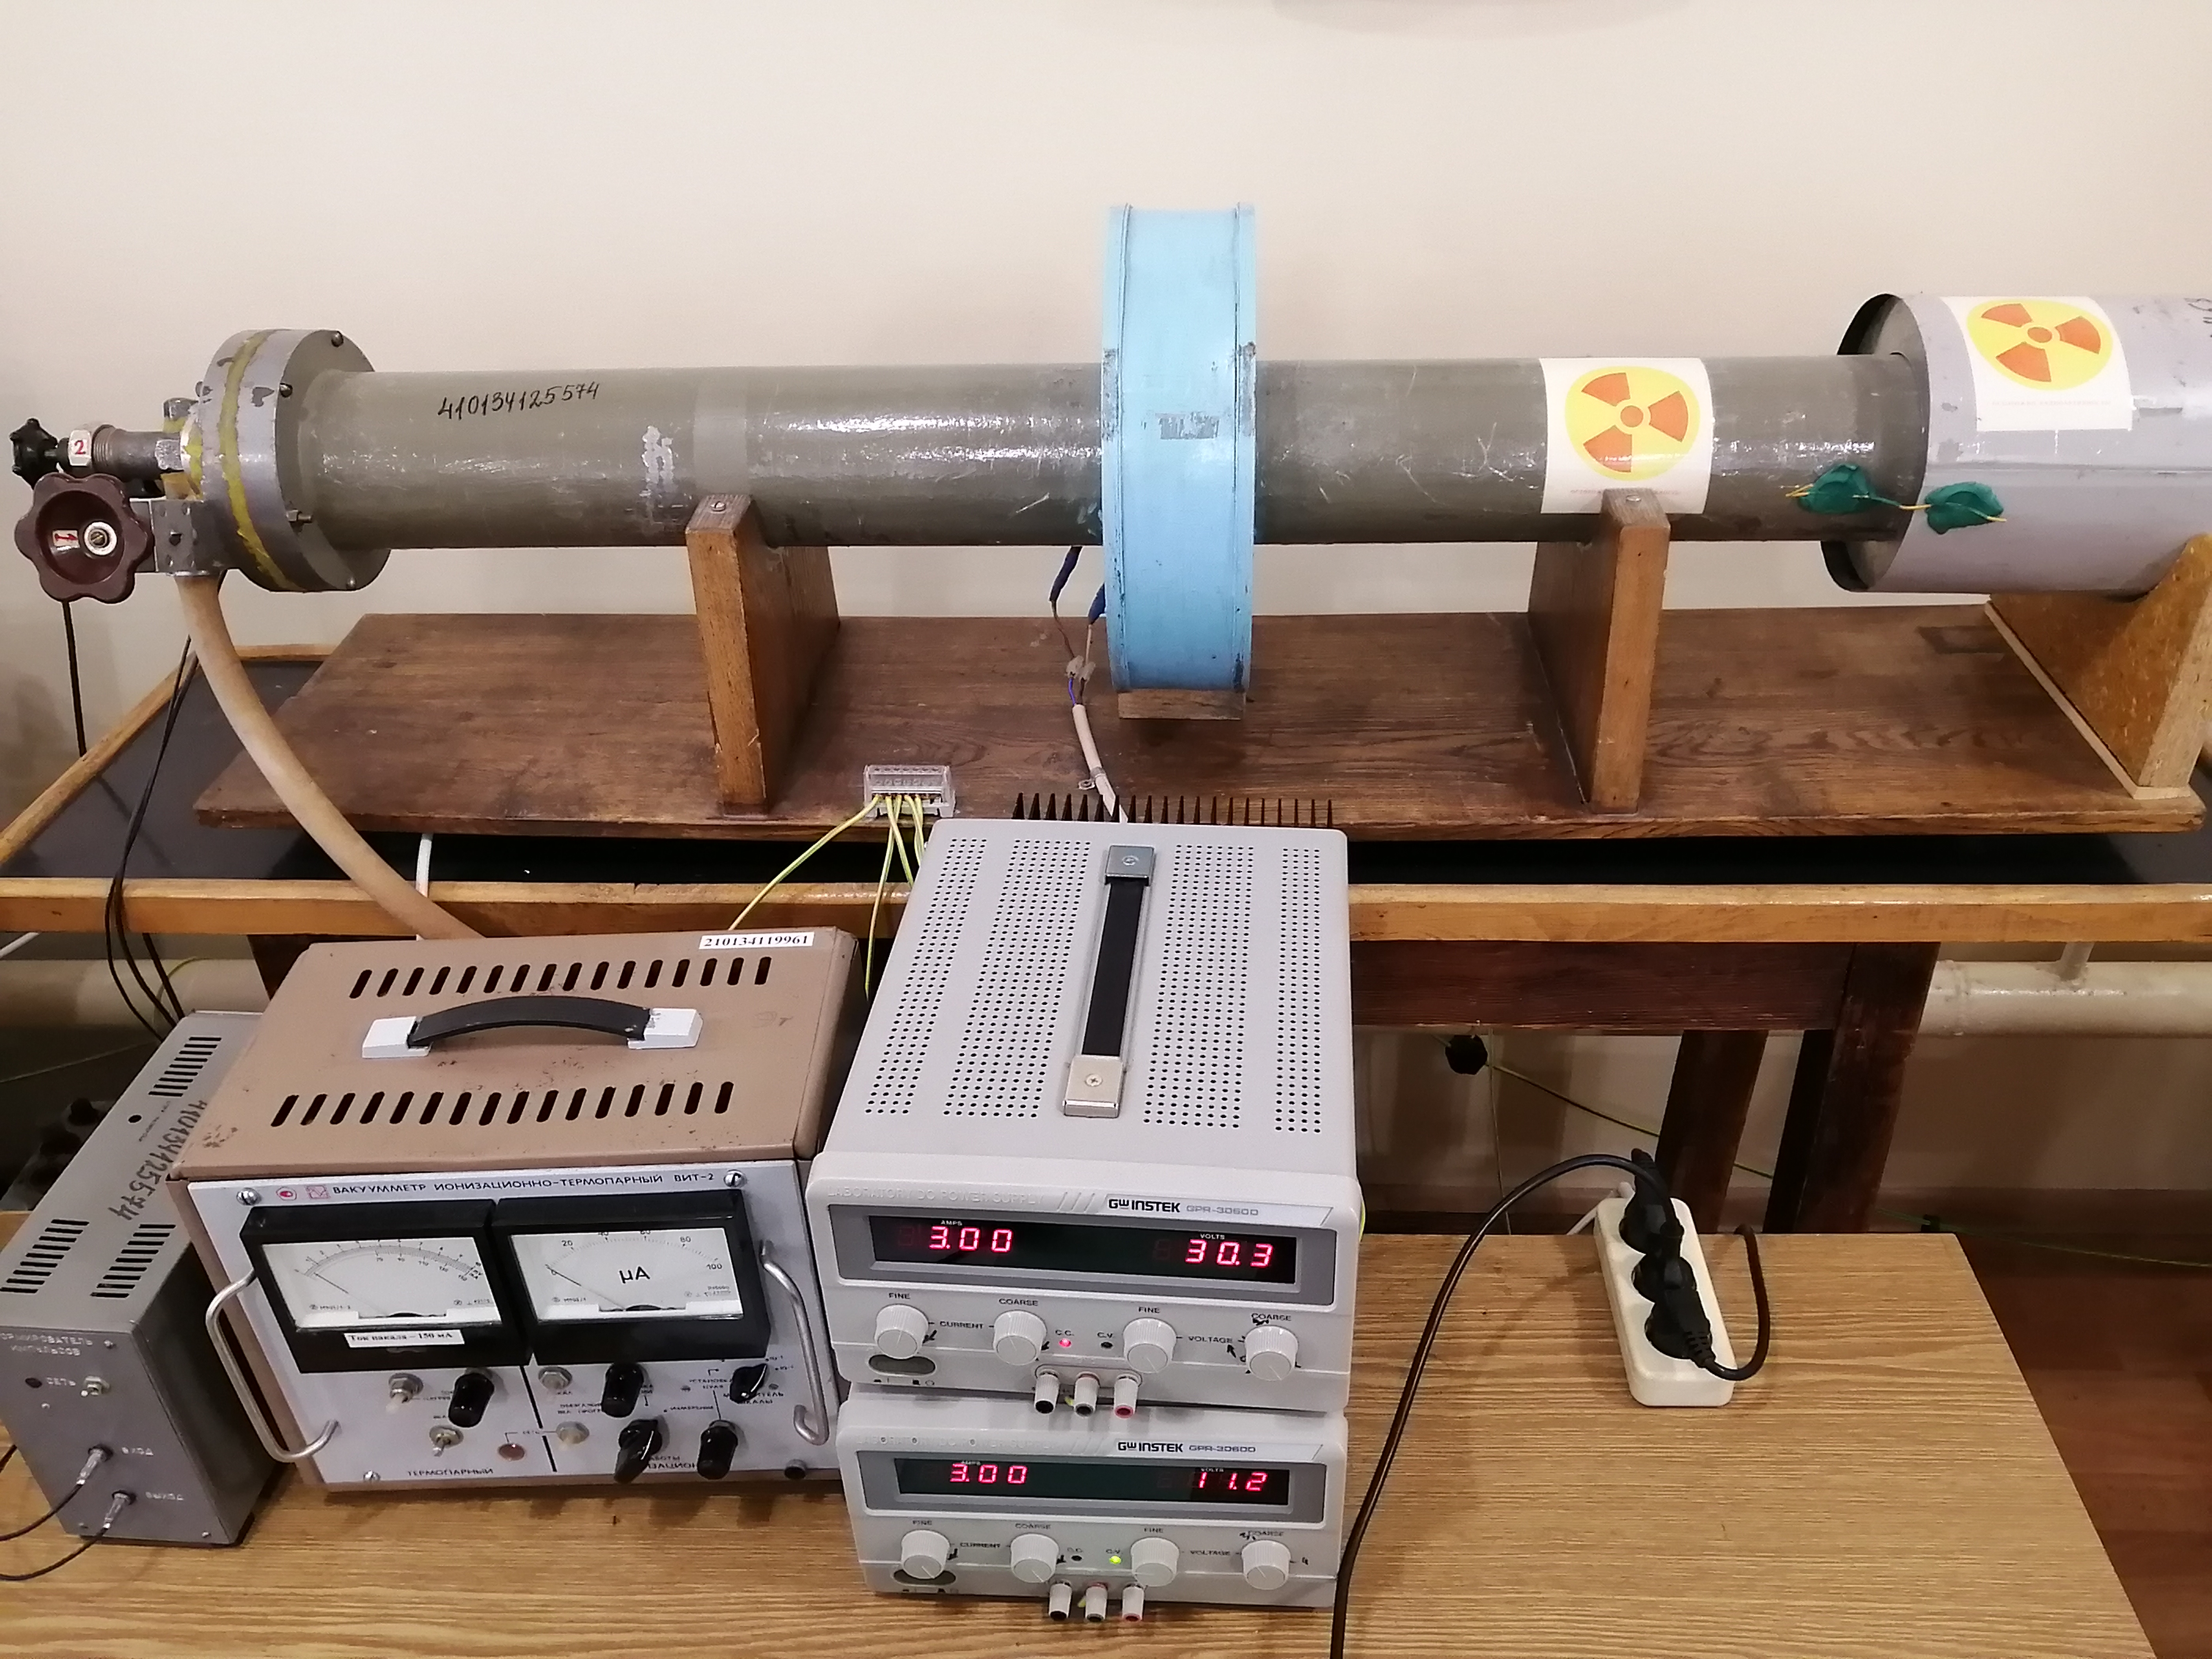
\includegraphics[width=0.9\linewidth]{photos/setup.jpg}
		\caption{Фотография установки.}
		\label{fig:setup}
	\end{figure}
	
	Измерения проводятся с использованием тиратрона ТГ3-01/1.3Б.
	
	В первой части работы измерения проводятся с помощью осциллографа. На графиках наблюдается зависимость напряжения $V_{\text{анод}}$ от напряжения катод-сетка $V_{\text{катод}}$. Напряжение $V_{\text{анод}}$ снимается с резистора $R = 100$ кОм, позволяя пересчитать его в ток анода $I_{\text{анод}}$.
	
	Во второй части работы измерения проводятся статически, с помощью вольтметров. Данные измерения повышают точность эксперимента, избавляя от инерционных эффектов, которые возникают при использовании осциллографа.
	
	На ВАХ тиратрона также оказывает влияение магнитное поле, так как приводит к ускорению отклонения рассеянных электронов. Для демонстрации эффекта используется неодимовый магнит.

	\newpage

	\section*{Результаты}
	
	\subsection*{Динамика}
	
	В соответствии с вышеописанной методикой получаем осциллограммы ВАХ тиратрона.

	\begin{figure}[H]
		\centering
		\begin{minipage}{0.49\textwidth}
			\centering
			\includegraphics[width=0.9\linewidth]{photos/ground.jpg}
		\end{minipage}%
		\begin{minipage}{0.49\textwidth}
			\centering
			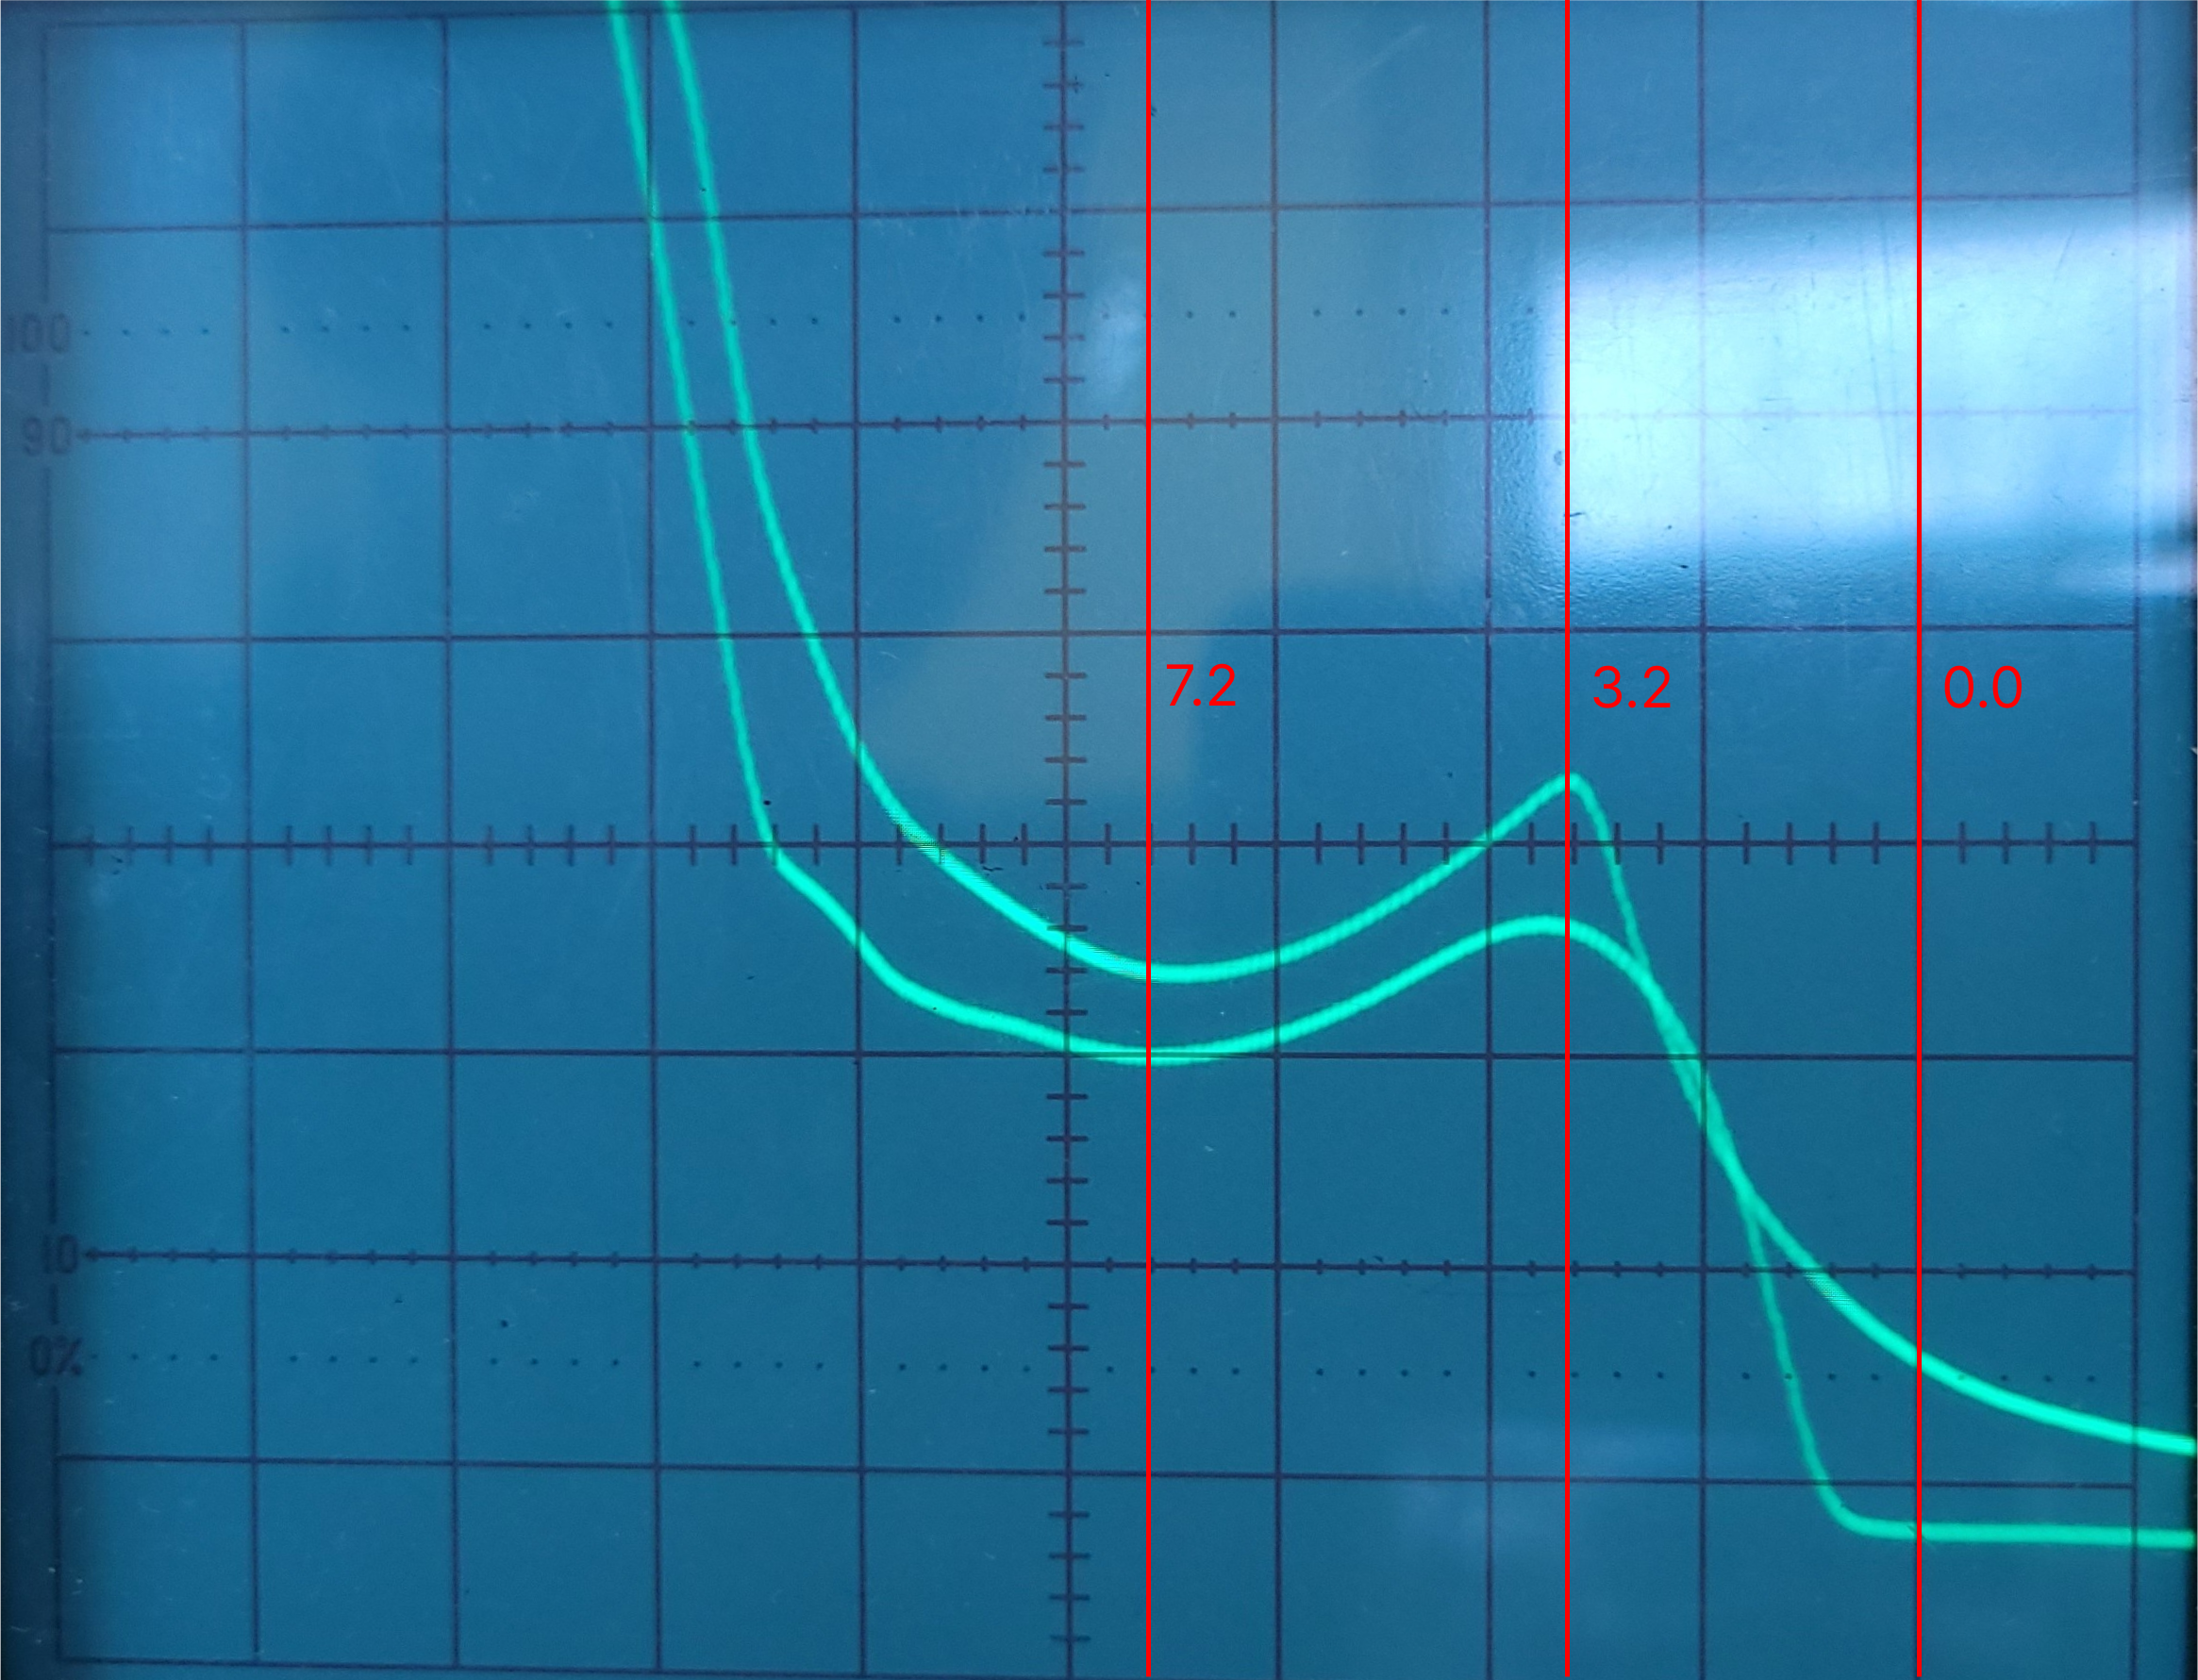
\includegraphics[width=0.9\linewidth]{photos/dyn.png}
		\end{minipage}
		\caption{Ноль (слева) и ВАХ тиратрона (справа).}
		\label{fig:dynamic}
	\end{figure}
	
	Из графиков определим: $V_{max} = (3.2 \pm 0.3)$ В, $V_{min} = (7.2 \pm 0.5)$ В.
	
	\begin{figure}[H]
		\centering
		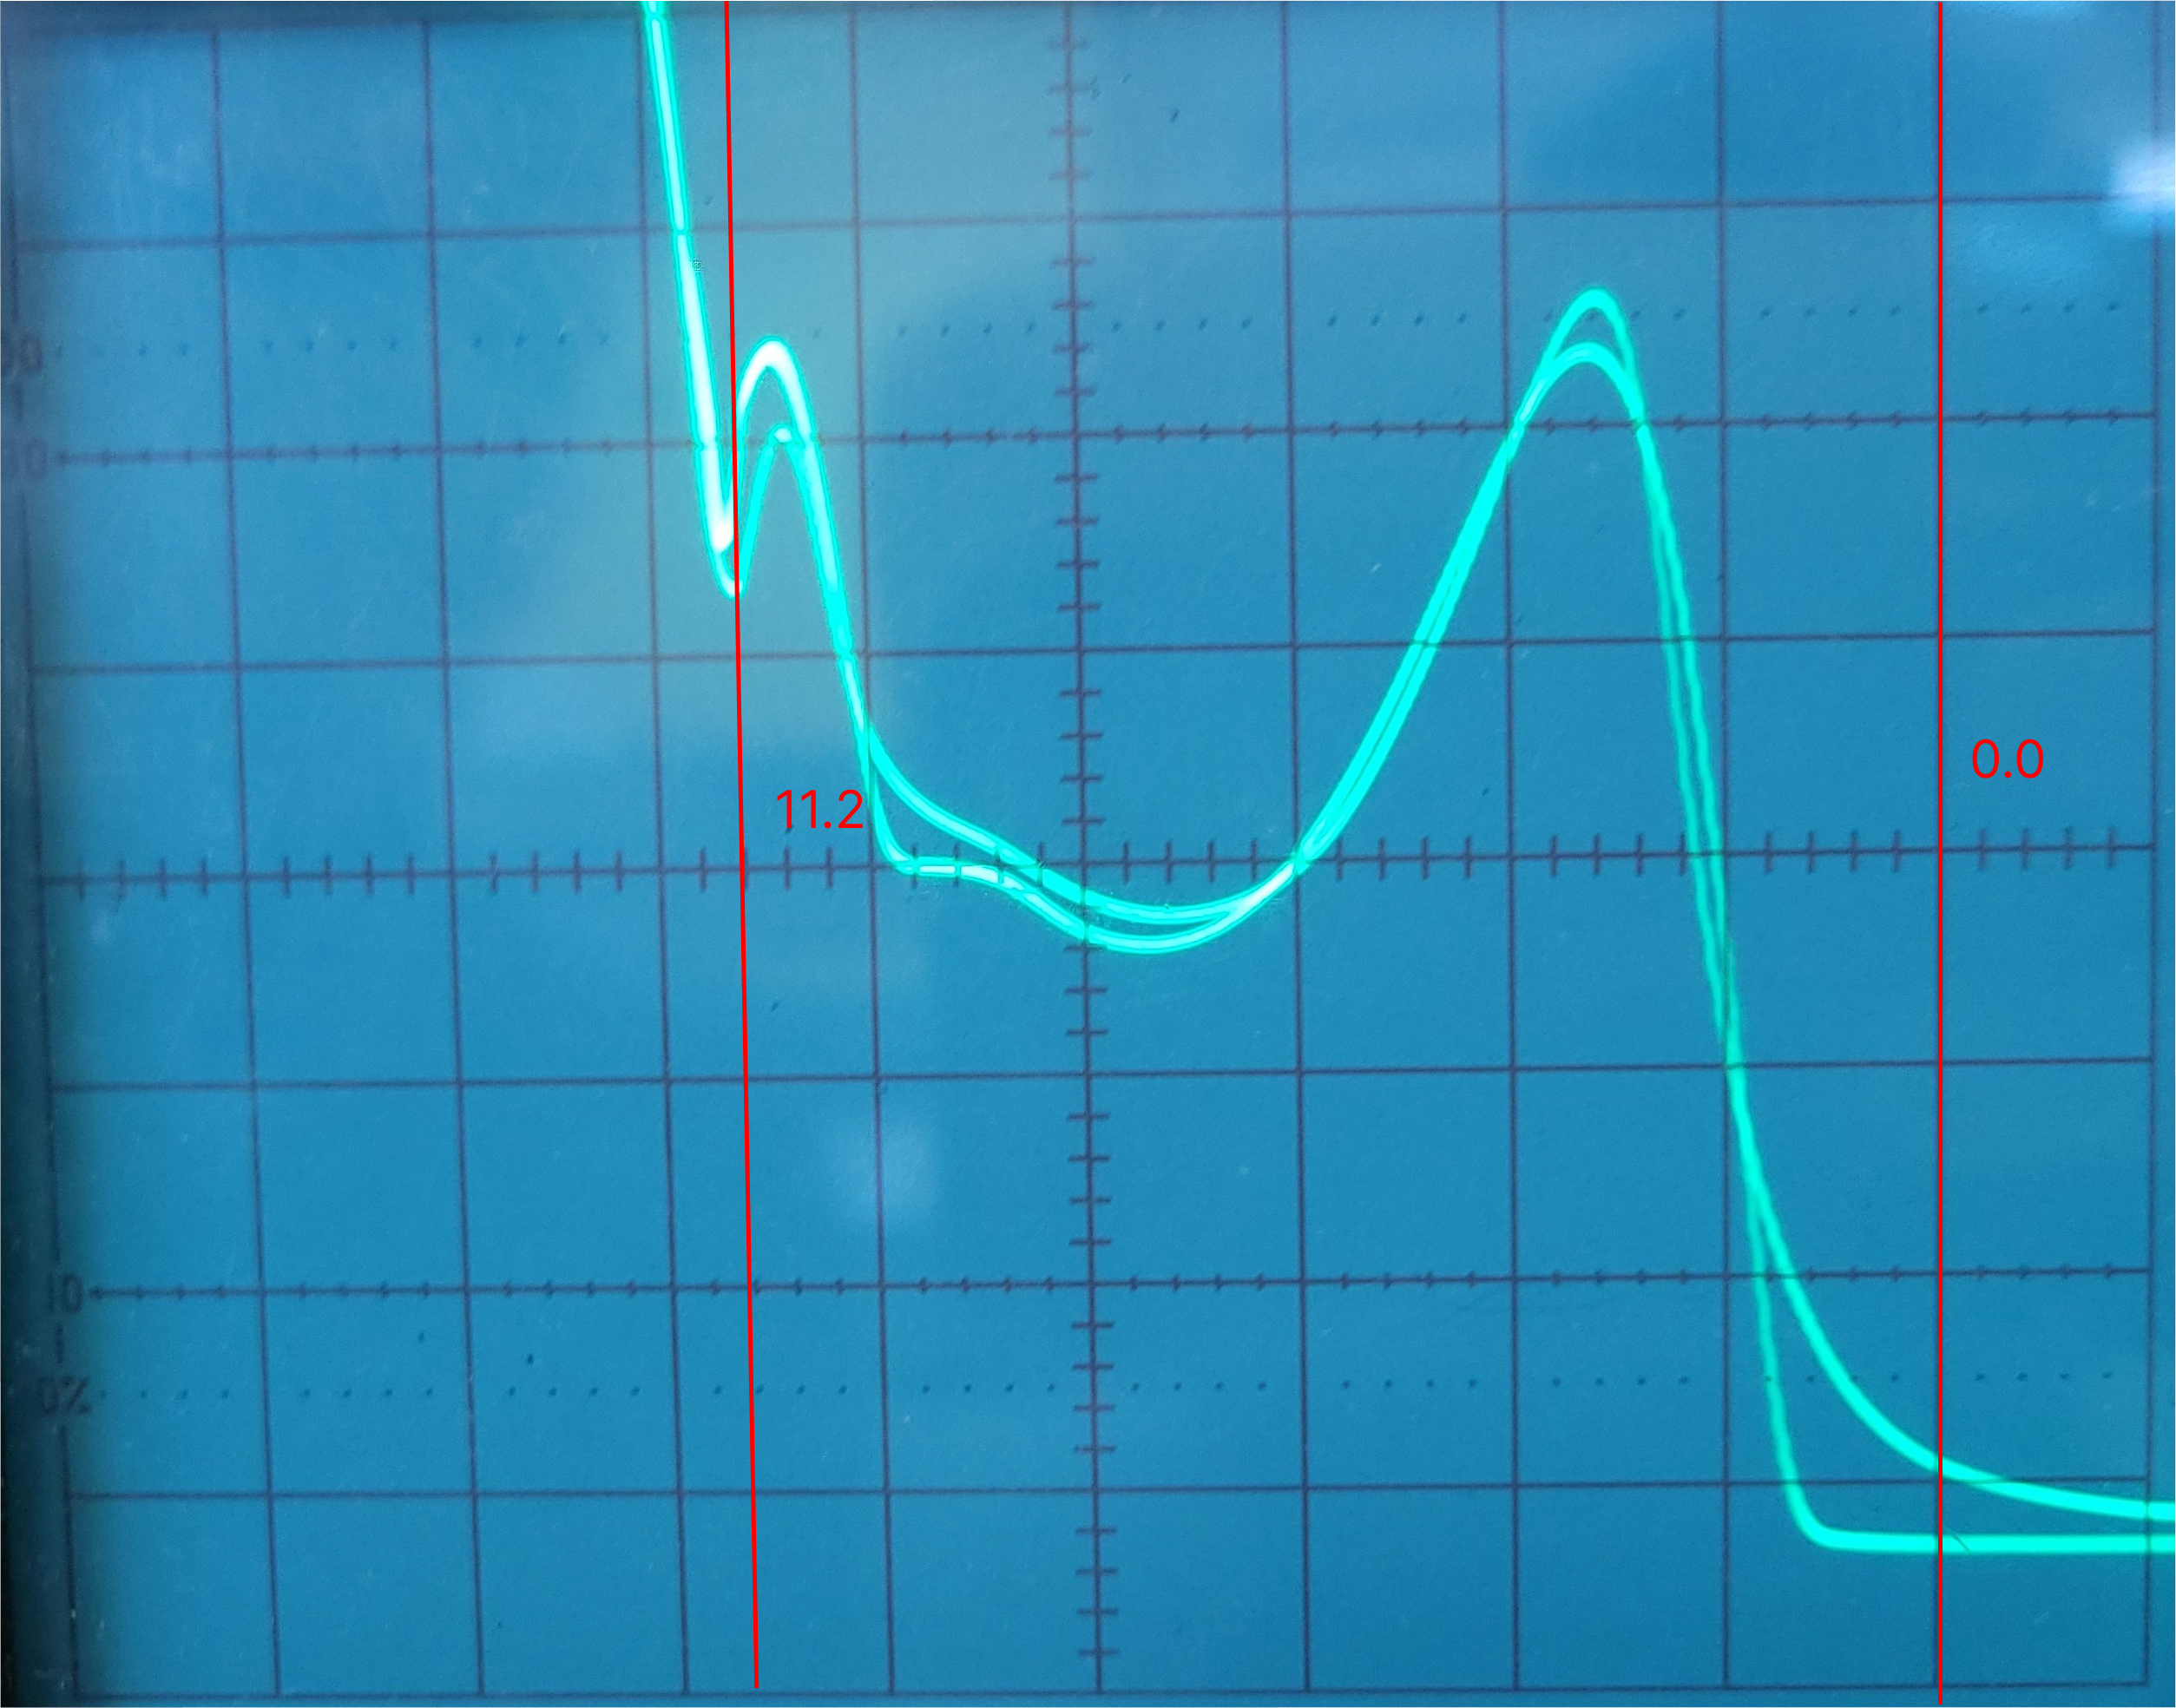
\includegraphics[width=0.5\linewidth]{photos/magnet.png}
		\caption{ВАХ тиратрона под воздействием магнита.}
		\label{fig:magnet}
	\end{figure}
	
	При поднесении к тиратрону неодимового магнита особенности ВАХ становятся более выраженными. Становится виден второй максимум. Благодаря этому можно найти напряжение пробоя: $V_{break} = (11.2 \pm 0.2)$ В.
	
	\newpage
	\subsection*{Статика}
	
	Измерения проводятся при двух значениях тока накала $V_{\text{накала}} = \{2.8 \text{ В}, 3.3 \text{ В}\}$.
	
	\begin{table}[H]
		\footnotesize
		\input{gen/data.tex}
		\caption{Данные зависимости анодного тока от напряжения катод-сетка.}
		\label{tab:data}
	\end{table}
	
	\begin{figure}[H]
		\centering
		\includegraphics[width=0.8\linewidth]{gen/static.pdf}
		\caption{ВАХ тиратрона.}
		\label{fig:static}
	\end{figure}
	
	Из графиков видно, что при высоком напряжении накала $V_{\text{накала}} = 3.3$ В эффект Рамзауэра выражен слабо. Минимум на этом графике определить невозможно, максимум совпадает с графиком $V_{\text{накала}} = 2.8$ В.
	Из графика определим $V_{max} = (2.5 \pm 0.1)$ В, $V_{min} = (7.5 \pm 0.2)$ В.
	
	Также рассчитаем $l$ и $U_0$ по формулам \eqref{eq:l_U0}:
	\begin{equation}
		l = (3.1 \pm 0.2) \text{ \AA}, \quad U_0 = (1.4 \pm 0.4) \text{ эВ}
	\end{equation}
	Оценка для $U_0$ неточна, так как в измерениях есть статистическая погрешность от контактной разности потенциалов.
	
	Оценим также потенциал ионизации:
	\begin{equation}
		I = U_{break} + U_0 \approx (12.6 \pm 0.5) \text{ эВ}
	\end{equation}
	
	Исходя из $I$ можем предполагать, что в тиратроне используется ксенон.
	
	Используя \eqref{eq:k} получим:
	\begin{equation}
		E_n = \frac{n^2 h^2}{8 m l^2} - U_0
	\end{equation}
	
	Для второго максимума получим $E_2 \approx 14$ эВ. Данное энергия выше энергии пробоя $E_{break} = (11.2 \pm 0.2)$ эВ, из чего следует, что наблюдаемый на рис. \ref{fig:magnet} максимум является иной особенностью ВАХ тиратрона.

	В соответствии с \eqref{eq:probability} построим $w(V)$:
	
	\begin{figure}[H]
		\centering
		\includegraphics[width=0.8\linewidth]{gen/probability.pdf}
		\caption{Зависимость вероятности рассеяния электрона от разгоняющего напряжения.}
		\label{fig:probability}
	\end{figure}
	
	Как и ожидалось, имеет смысл рассматривать только $V_{\text{накала}} = 2.8$ В. На этом графике мы наблюдаем минимум и максимум вероятности рассеяния $w(V)$. 
	
	\section*{Заключение и выводы}
	
	В работе подтверждено существования эффекта Рамзауэра.
	
	Получено оценка размера атома в тиратроне $l = (3.1 \pm 0.2)$ \AA. Оценены значения глубины потенциальной ямы $U_0 = (1.4 \pm 0.4)$ эВ и энергии ионизации $I = (12.6 \pm 0.5)$ эВ. По энергии ионизации определен инертный газ в тиратроне: ксенон. Табличное значение $l = 2.8$ \AA.

	Для повышения точности результатов можно провести измерения контактного потенциала, избавившись от статистической погрешности $U_0$ и $I$, составляющей $<0.5$ В.
\end{document}
